\onecolumn

\appendix
\label{app:detailed_results}

\section{Detailed Results}
\label{app:detailed_tables}

\subsection{Token Size Distribution}
\label{app:token_size}

The distribution of token lengths provides important insights into tokenizer design and potential efficiency. Figure~\ref{fig:token_size_comparison} presents a line plot comparing the percentage of vocabulary by token length across tokenizers.

\begin{figure*}[htbp]
    \centering
    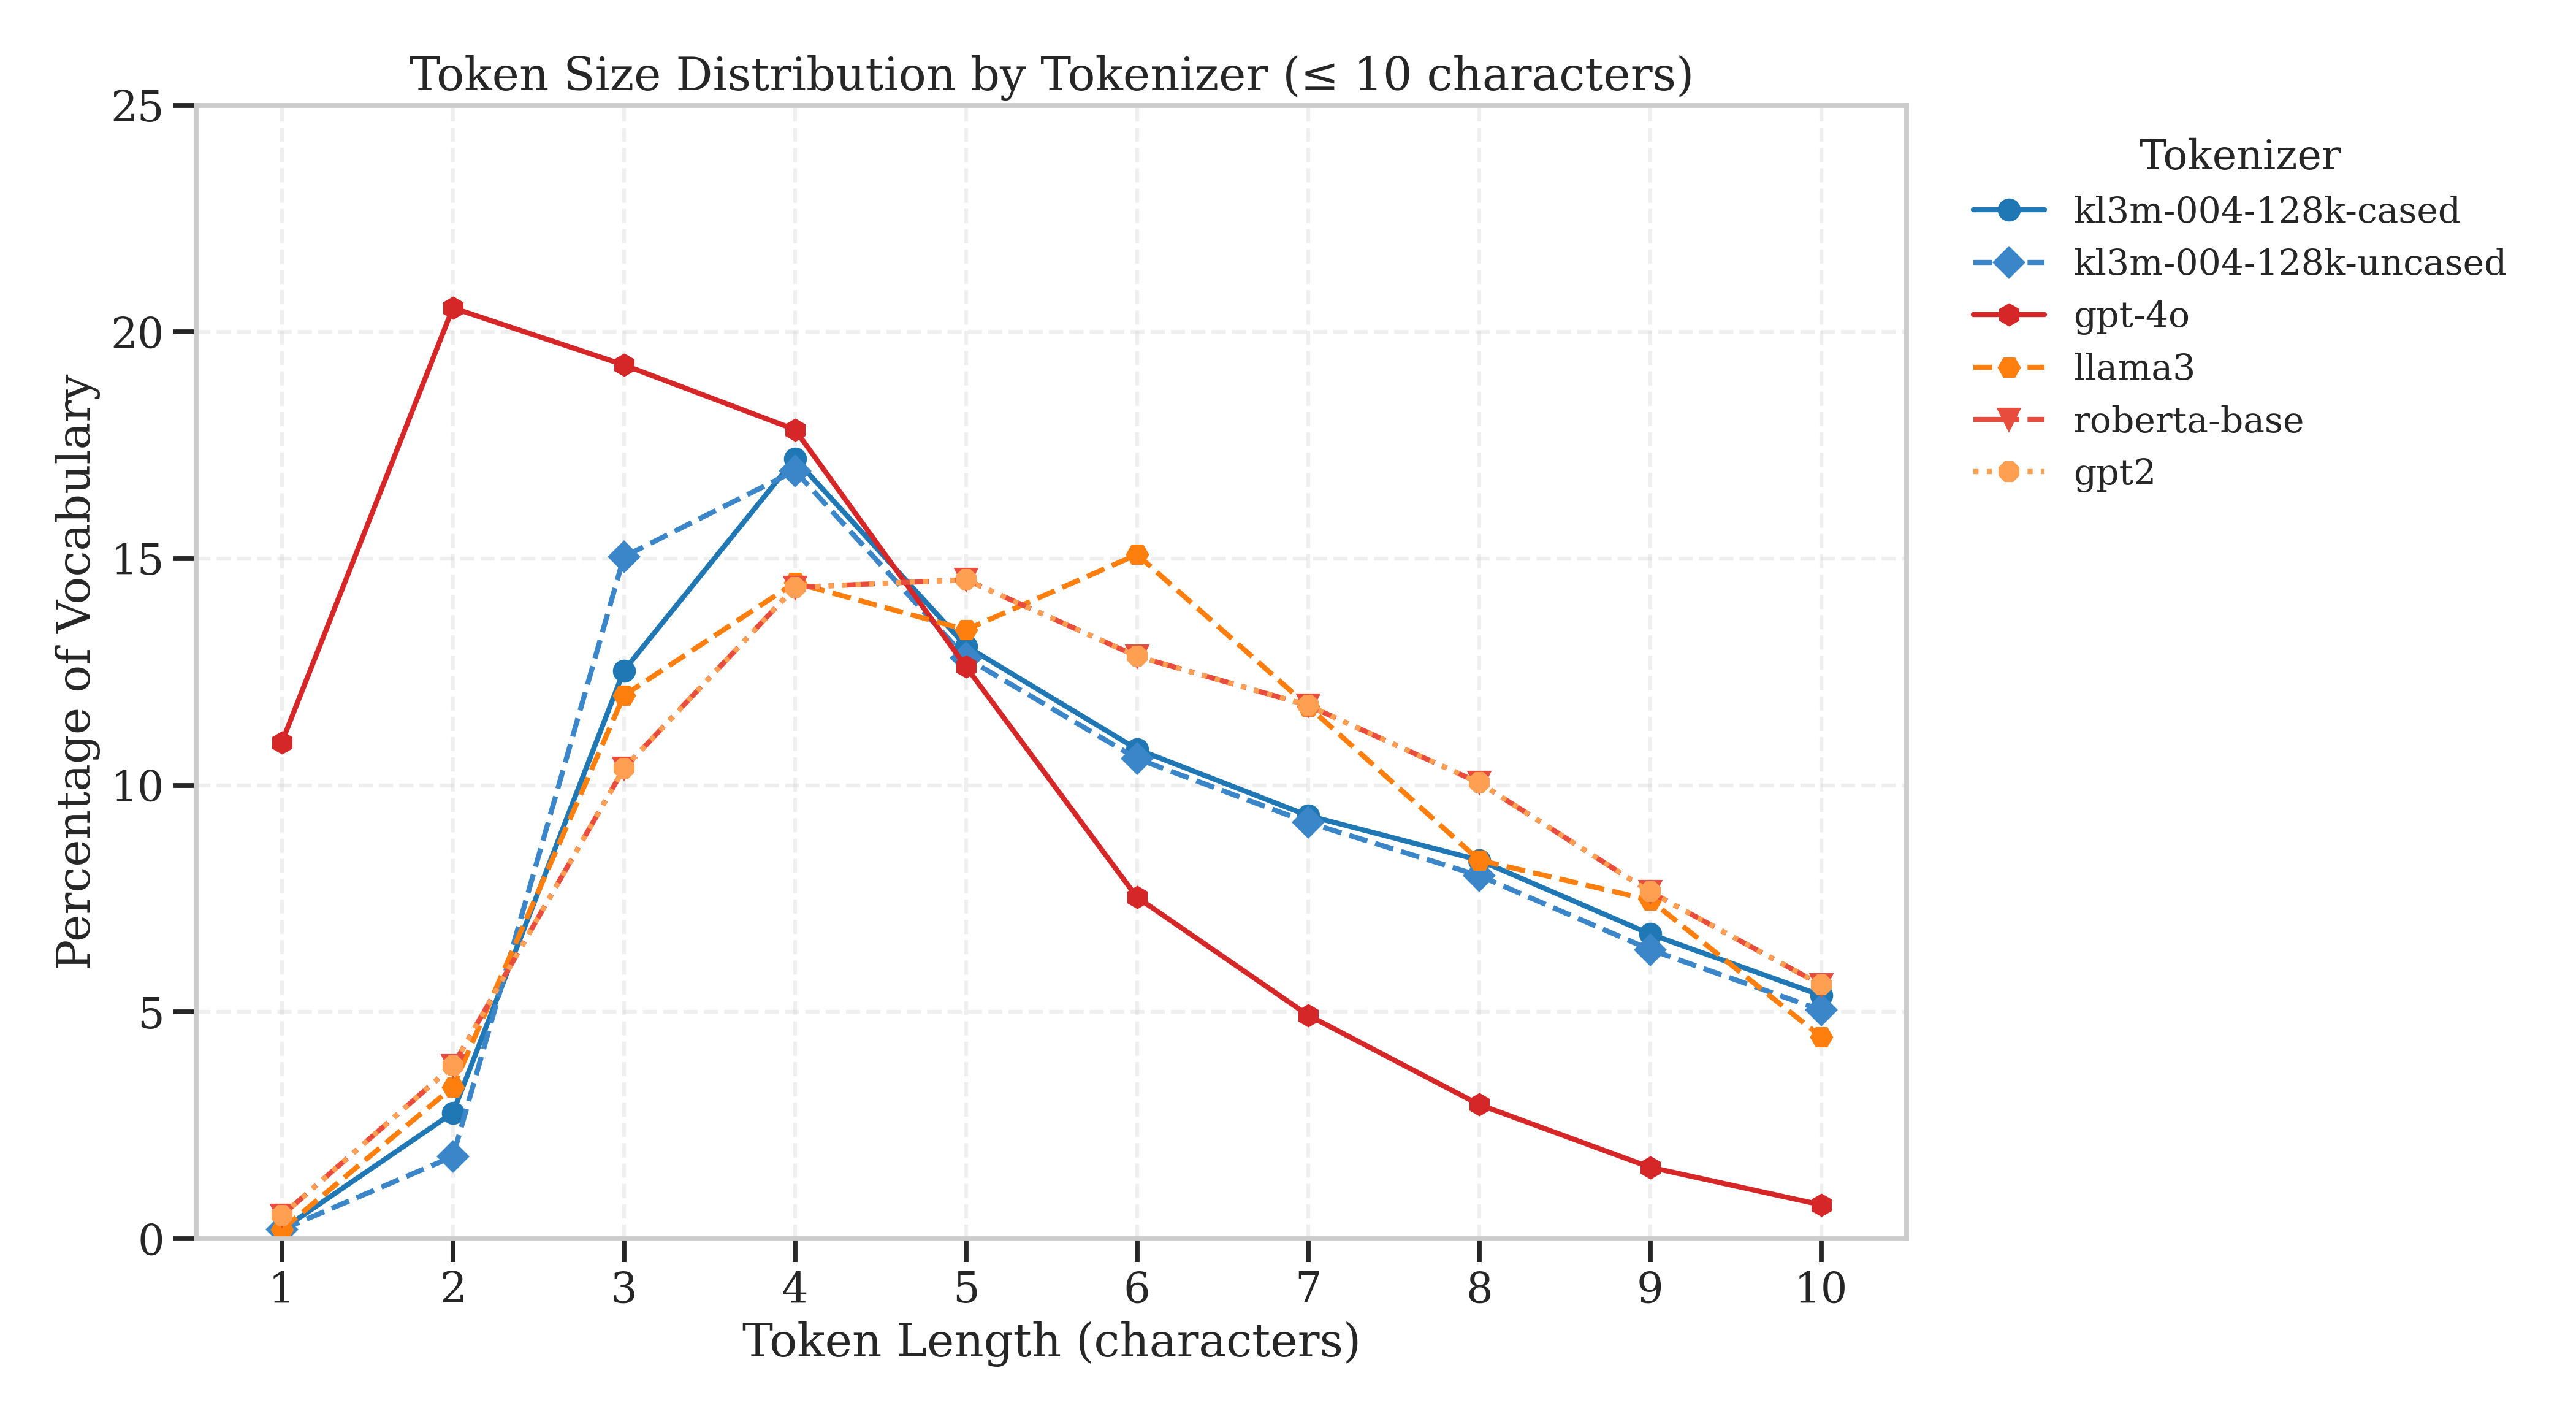
\includegraphics[width=0.95\textwidth]{figures/token_size_comparison.png}
    \caption{Percentage of vocabulary by token length across tokenizers. KL3M tokenizers show higher percentages of medium-length tokens (3-6 characters) compared to other tokenizers.}
    \label{fig:token_size_comparison}
\end{figure*}

% Token size distribution table
\begin{table*}[htbp]
\centering
\caption{Token size distribution (percentage of vocabulary by character length). Note: For tiktoken models like \texttt{gpt-4o}, only a subset of tokens can be individually decoded, so statistics are based on a partial sample.}
\label{tab:token-size-distribution}
\small
\begin{tabular}{lrrrrrr}
\toprule
Length & kl3m\mbox{-}004\mbox{-}128k\mbox{-}cased & kl3m\mbox{-}004\mbox{-}128k\mbox{-}uncased & gpt\mbox{-}4o & llama3 & roberta\mbox{-}base & gpt2 \\
\midrule
1 & 0.2\% & 0.2\% & 10.9\% & 0.2\% & 0.5\% & 0.5\% \\
2 & 2.8\% & 1.8\% & 20.5\% & 3.3\% & 3.8\% & 3.8\% \\
3 & 12.5\% & 15.0\% & 19.3\% & 12.0\% & 10.4\% & 10.4\% \\
4 & 17.2\% & 16.9\% & 17.8\% & 14.5\% & 14.4\% & 14.4\% \\
5 & 13.1\% & 12.8\% & 12.6\% & 13.4\% & 14.5\% & 14.5\% \\
6 & 10.8\% & 10.6\% & 7.5\% & 15.1\% & 12.8\% & 12.8\% \\
7 & 9.3\% & 9.2\% & 4.9\% & 11.7\% & 11.8\% & 11.8\% \\
8 & 8.3\% & 8.0\% & 3.0\% & 8.4\% & 10.1\% & 10.1\% \\
9 & 6.7\% & 6.4\% & 1.6\% & 7.5\% & 7.6\% & 7.7\% \\
10 & 5.4\% & 5.0\% & 0.7\% & 4.5\% & 5.6\% & 5.6\% \\
\midrule
Total $\leq 5$ & 45.8\% & 46.8\% & 81.2\% & 43.4\% & 43.6\% & 43.6\% \\
Total 6-10 & 40.6\% & 39.2\% & 17.7\% & 47.1\% & 47.9\% & 47.9\% \\
Total $\leq 10$ & 86.3\% & 86.0\% & 99.0\% & 90.5\% & 91.5\% & 91.5\% \\
\bottomrule
\end{tabular}
\end{table*}

KL3M tokenizers, particularly the kl3m-004-128k variants, have a more balanced distribution with a higher percentage of medium-length tokens (3-6 characters). In contrast, \texttt{gpt-4o} has a significantly higher percentage of short tokens (1-2 characters), with over 31% of its vocabulary consisting of tokens of 1-2 characters in length, compared to only 2-3% for KL3M tokenizers.

\subsection{Tokenization Efficiency Visualizations}
\label{app:token_efficiency_charts}

Tokenization efficiency, measured as tokens per character (TPC), represents the inverse of compression ratio. Lower TPC values indicate better compression and higher efficiency, as fewer tokens are needed to encode the same amount of text. Figure~\ref{fig:token_efficiency_bars} provides a visual comparison of tokenization efficiency across datasets for different tokenizers.

\begin{figure*}[htbp]
    \centering
    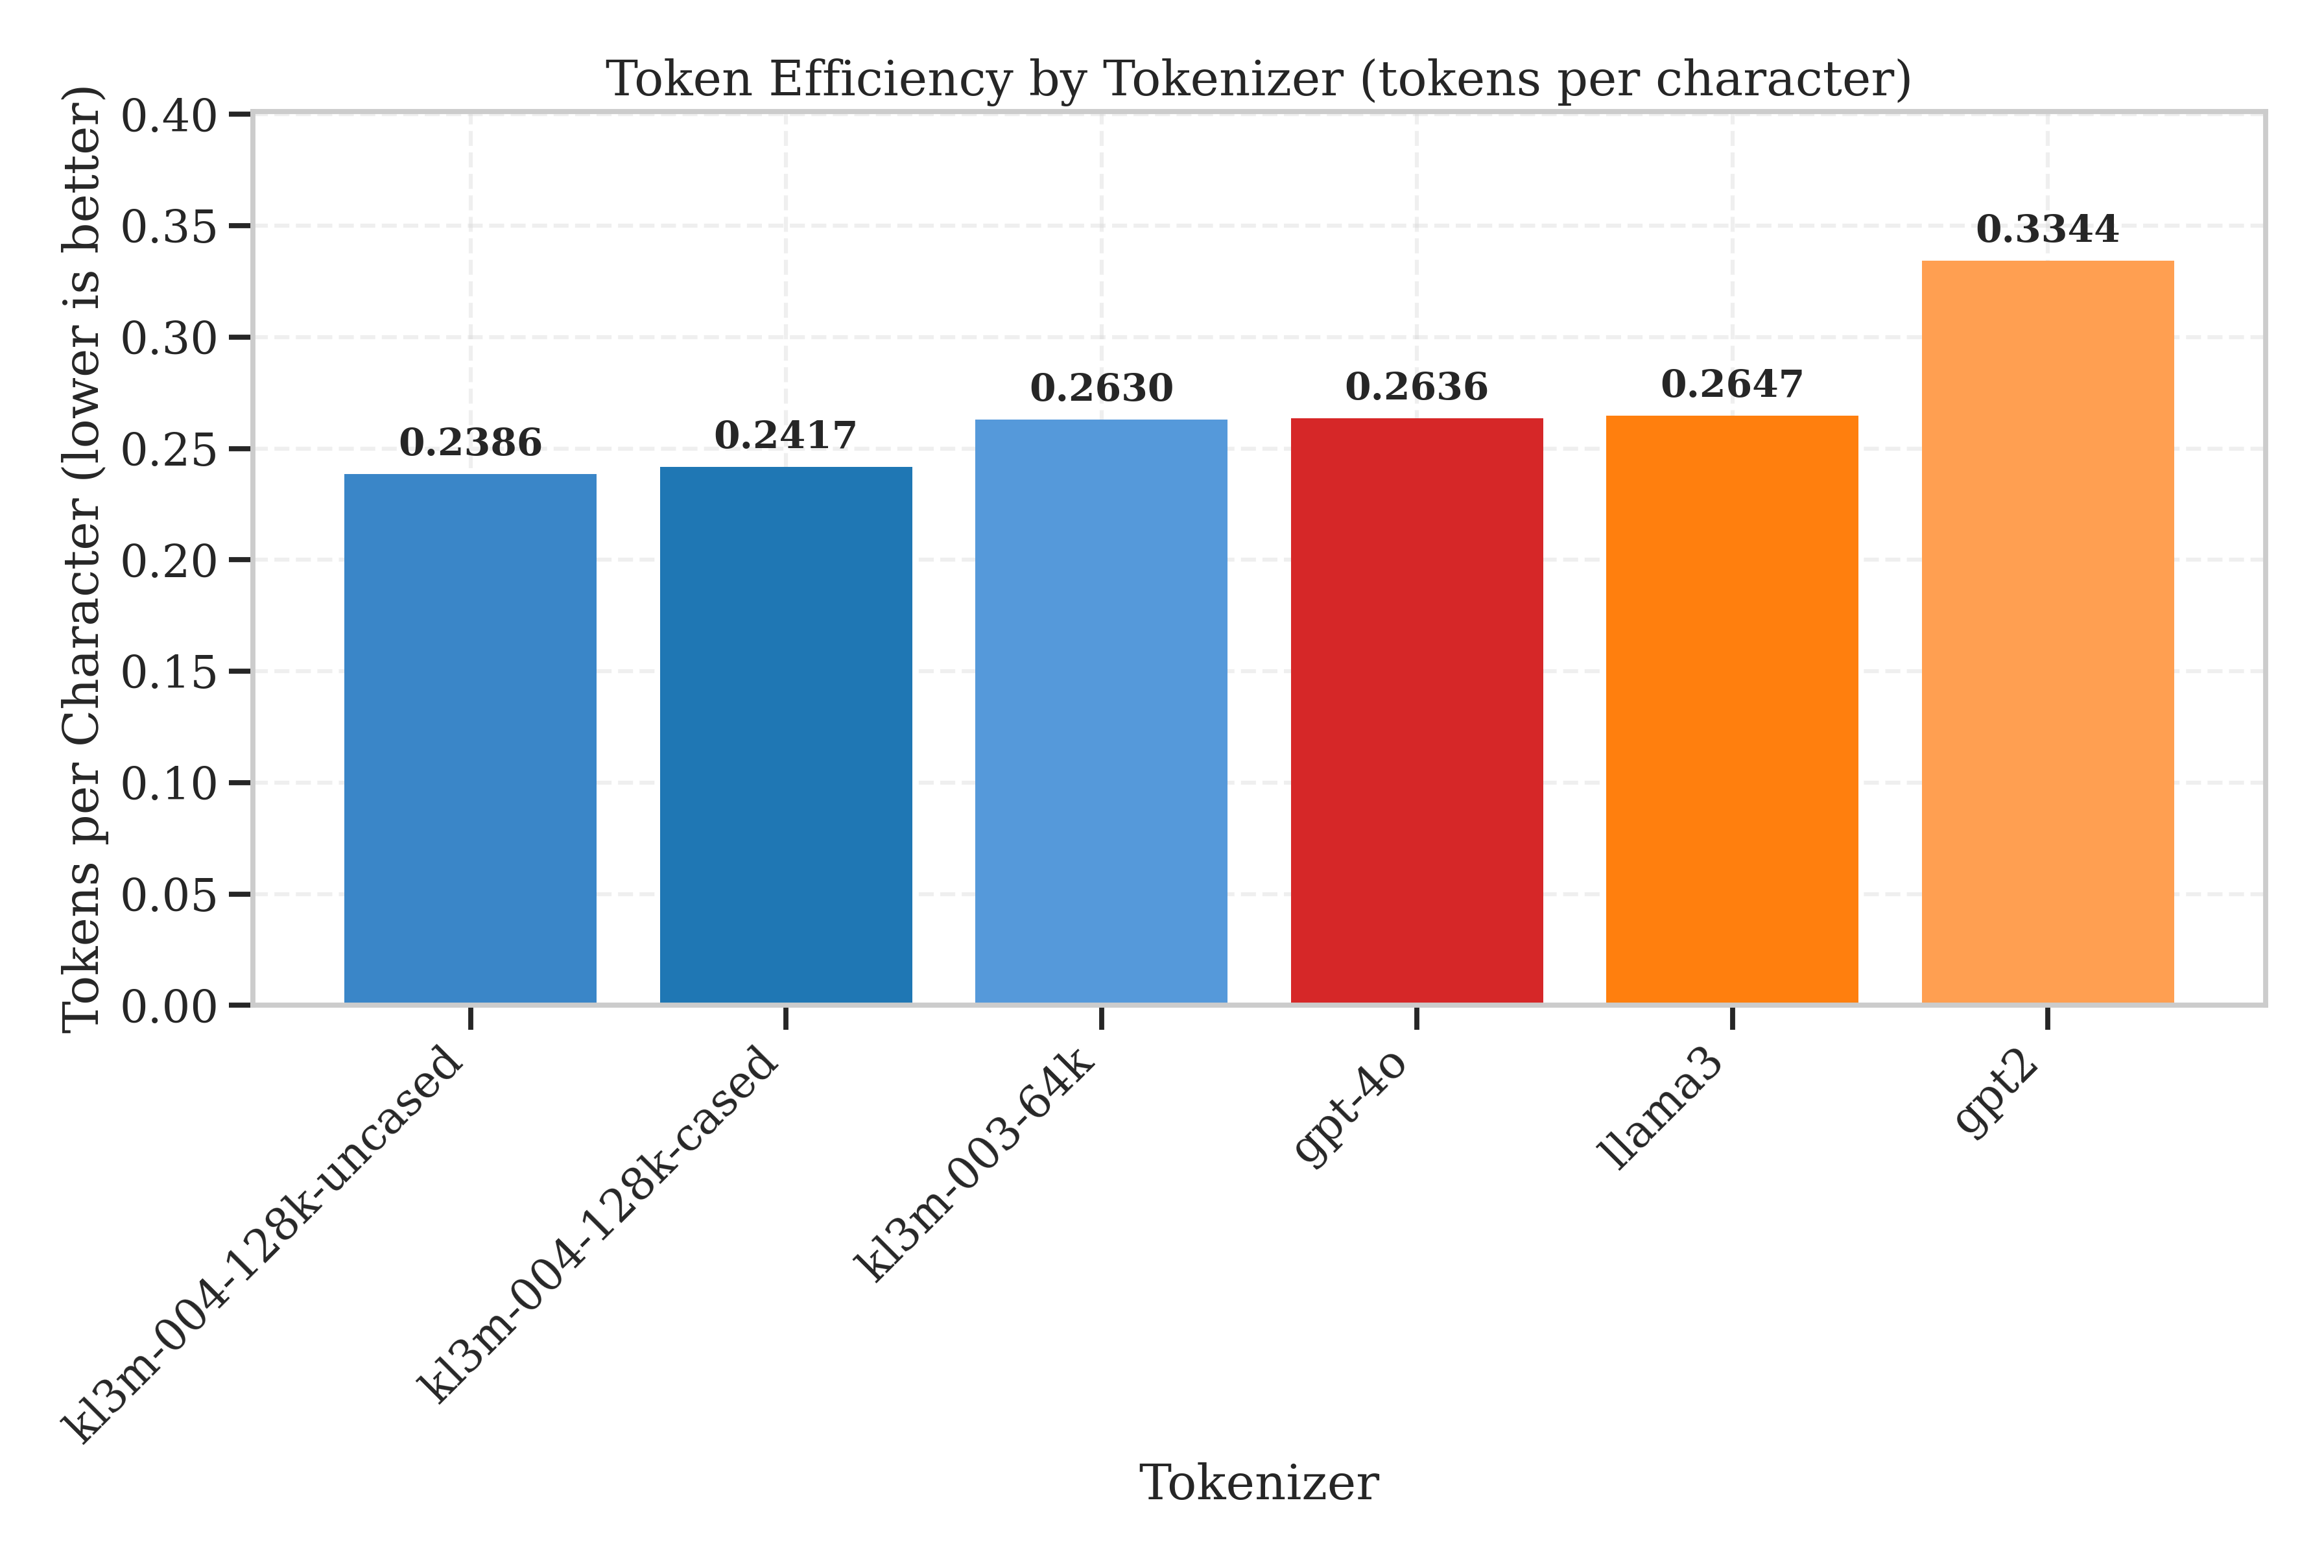
\includegraphics[width=0.85\textwidth]{figures/token_efficiency_bars.png}
    \caption{Tokenization efficiency (tokens per character) across datasets. Lower values indicate higher efficiency. KL3M tokenizers consistently demonstrate higher efficiency, particularly for domain-specific content like US Code and Congressional Hearings.}
    \label{fig:token_efficiency_bars}
\end{figure*}

\subsection{Total Token Count Comparison}
\label{app:token_count}

Table~\ref{tab:token-count} presents the absolute token counts for each tokenizer across the different datasets, providing a concrete measure of the efficiency improvements offered by the KL3M tokenizers.

% LaTeX table for token count analysis
\begin{table}[ht]
\centering
\caption{Total token count across datasets\\\small \textit{Note: Lower values indicate more efficient tokenization (fewer tokens to represent the same text).}}
\label{tab:token-count}
\small
\begin{tabular}{lrrrrrr}
\toprule
Dataset & kl3m\mbox{-}004\mbox{-}128k\mbox{-}cased & kl3m\mbox{-}004\mbox{-}128k\mbox{-}uncased & kl3m\mbox{-}003\mbox{-}64k & gpt\mbox{-}4o & llama3 & gpt2 \\
\midrule
Congressional Hearings & 308,169 & \textbf{299,954} & 377,458 & 333,702 & 332,791 & 506,115 \\
Court Documents & 23,682 & \textbf{23,260} & 25,116 & 25,674 & 25,798 & 30,454 \\
General Content & 22,424 & \textbf{22,164} & 24,237 & 22,167 & 22,522 & 23,068 \\
SEC Filings & 243,580 & \textbf{242,057} & 256,913 & 265,078 & 267,267 & 499,126 \\
US Code & 45,099 & \textbf{44,957} & 46,732 & 52,684 & 52,689 & 50,962 \\
\midrule
Total & 642,954 & \textbf{632,392} & 730,456 & 699,305 & 701,067 & 1,109,725 \\
\bottomrule
\end{tabular}
\end{table}
